\lecture{7}{10.09}
\begin{notation}
    美伐他汀从青霉菌中提取、有致癌效应

    由美伐他汀所延伸的洛伐他汀活性更大、但毒性也更大

    洛伐他汀:从红曲霉菌和土曲霉菌中提取
\end{notation}
由洛伐他汀为前体,在体内代谢产生多种活性代谢物,再根据这些代谢物合成新的药物
\begin{notation}
    由某些活性化合物经过一次反应,得到的物质可能失去活性
\end{notation}
人工合成他汀类化合物的需求:负责构效关系的基团保持不变

他汀类药物的构效关系:六元开环/闭环的一个基团
\begin{notation}
    辉瑞开发的阿伐他汀副作用最小,销售最好
\end{notation}
他汀类药物的不良反应:

1. 肌毒性:与贝特类药物共用时更易导致横纹肌溶解

2. 会导致肝脏转氨酶升高
\subsubsection{研究任务}%
\label{subsub:研究任务-}
1. 为有效利用现有化学药物提供理论基础

2. 为生产化学药物提供经济合理的方法和工艺

3. 探索开发新药的途径和方法
\begin{notation}
    途径:

    1. 意外发现

    2. 筛选

    3. 药物设计

    设计的4个阶段:

    1. 生物靶点的选择

    2. 监测系统的确定

    3. 先导化合物的发现

    4. 先导化合物的优化
\end{notation}
\subsubsection{药化与其他学科的关系}%
\label{subsub:化与其他学科的关系-}
药学同化学、生命科学同为药学各学科的基础

\subsection{药物化学的历史和现状}%
\label{sub:药物化学的历史和现状}
\subsubsection{历史}%
\label{subsub:历史}
\begin{notation}
    药物化学的发展史是药物研究和开发的历史,是由粗到精、由盲目到自觉、由经验性的试验到科学合理的设计过程
\end{notation}
\[
    \begin{cases}
        \text{发现阶段:19世纪末-20世纪30年代}\\
        \text{发展阶段:20世纪30至60阶段}\\
        \text{设计阶段:20世纪60年代至今}
    \end{cases}
.\] 
\begin{figure}[htpb]
    \centering
    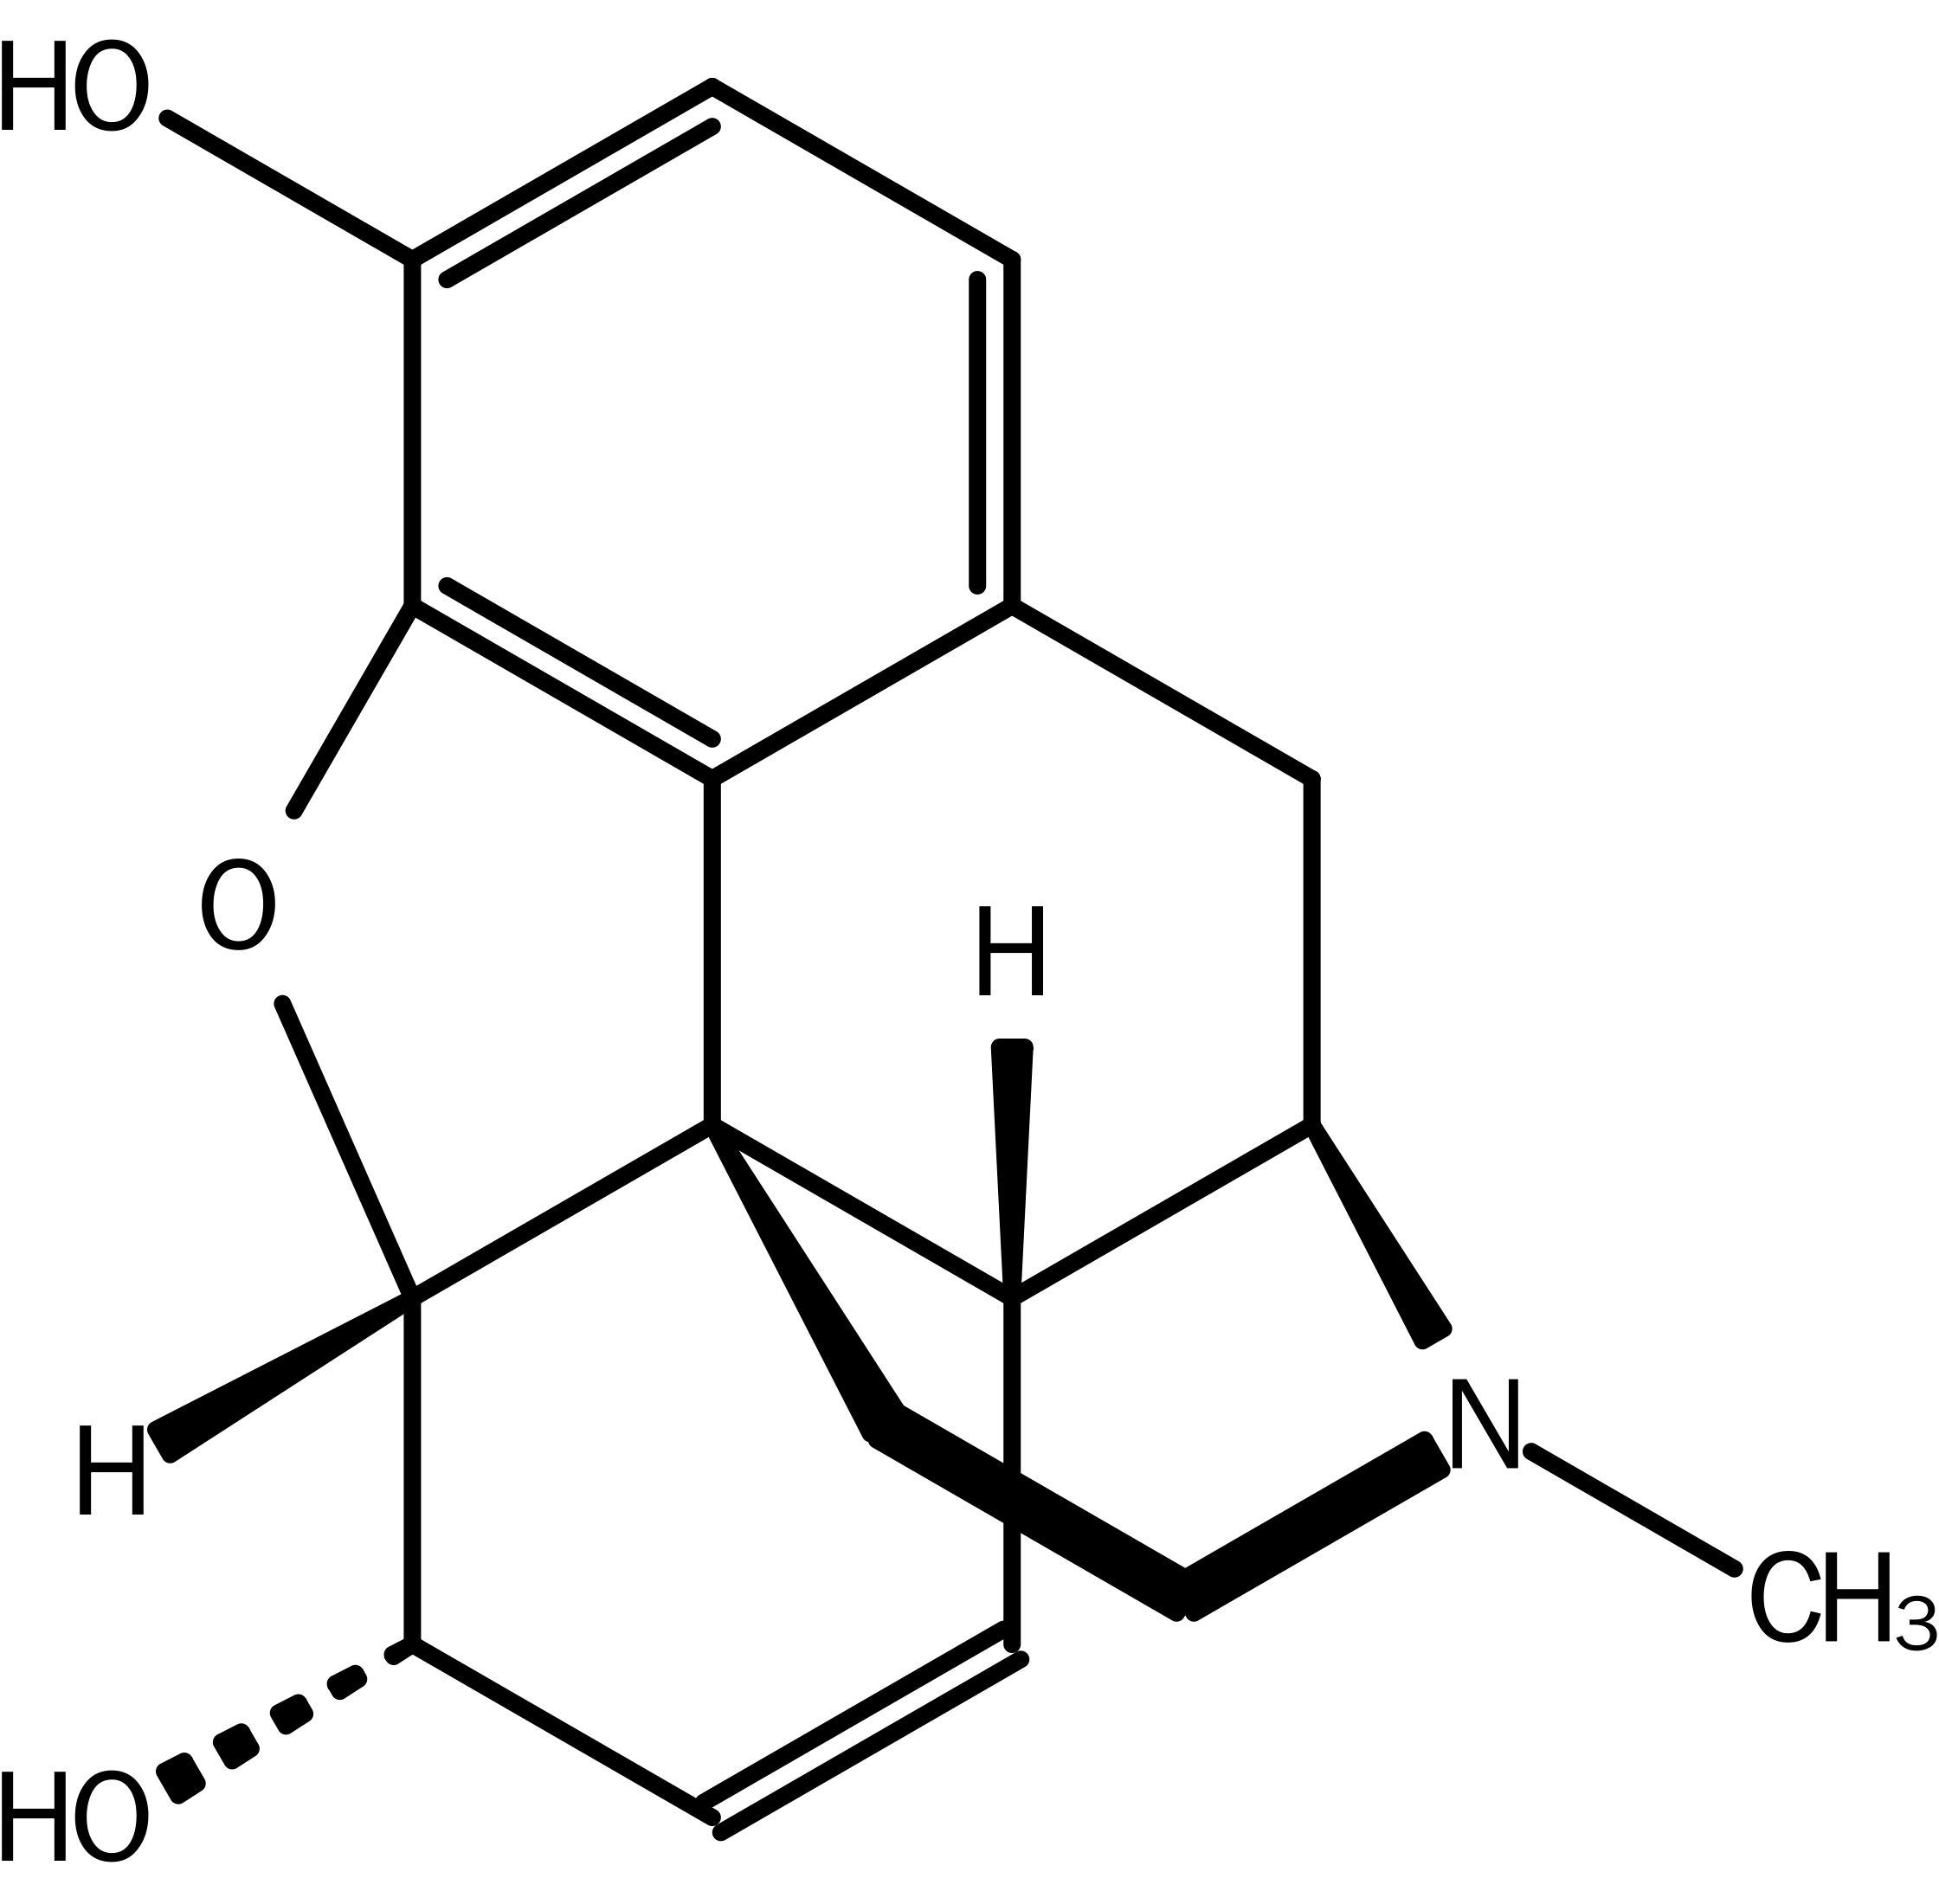
\includegraphics[width=0.25\textwidth]{fig/Morphine}
    \caption{Morphine}
    \label{fig:fig-Morphine}
\end{figure}
\begin{notation}
    发现阶段:

    特征:从动植物中分离、纯化、测定

    高光时刻:“神药”阿司匹林的合成

    1884:合成氨基比林

    1886:合成衍生物匹拉米洞

    1886:发现苯胺、乙酰苯胺可镇痛

    1887:合成衍生物非那西丁

    去痛片/大白片:氨基比林+非那西丁+咖啡因+苯巴比妥

    1856:提取古柯碱

    1865:古柯碱水解得到爱康宁、苯甲酸、甲醇

    1890:苯佐卡因合成,有局麻作用

    1897:合成优卡因,麻醉效果比古柯碱好

    1904:艾因霍恩合成普鲁卡因
\end{notation}
\begin{notation}
    发展阶段:

    药物发展的黄金时期,与有机化学的理论和实验技术的发展密切相关

    代表:
    
    甾体激素类化合物:“四环素”

    抗生素:青霉素

    构效关系理论得到确定
\end{notation}

